\documentclass{article}

\usepackage{fancyhdr}
\usepackage{extramarks}
\usepackage{amsmath}
\usepackage{amsthm}
\usepackage{amsfonts}
\usepackage{tikz}
\usepackage[plain]{algorithm}
\usepackage{algpseudocode}
\usepackage{listings}
\usetikzlibrary{automata,positioning}

%
% Basic Document Settings
%

\topmargin=-0.45in
\evensidemargin=0in
\oddsidemargin=0in
\textwidth=6.5in
\textheight=9.0in
\headsep=0.25in

\linespread{1.1}

\pagestyle{fancy}
\chead{\hmwkClass\ : \hmwkTitle}
\rhead{  }
\lhead{}
\lfoot{\lastxmark}
\cfoot{\thepage}

\renewcommand\headrulewidth{0.4pt}
\renewcommand\footrulewidth{0.4pt}

\setlength\parindent{0pt}

%
% Create Problem Sections
%

	



%
% Homework Details
%   - Title
%   - Due date
%   - Class
%   - Section/Time
%   - Instructor
%   - Author
%
\newcommand{\hmwkTitle}{Rapport Final}
\newcommand{\hmwkDueDate}{15/12/2019 à 0h00}
\newcommand{\hmwkClass}{Systèmes Microprogrammés}
\newcommand{\hmwkClassTime}{Groupe 2}
\newcommand{\hmwkClassInstructor}{}

\newcommand{\hmwkAuthorName}{CHAYMAE  FAZAZI-IDRISSI}
\newcommand{\autre}{ZHAO Yue}
\newcommand{\auttre}{ZHANG Quan}
%
% Title Page
%

\title{
    \vspace{1in}
    \textmd{\textbf{\hmwkClass}}\\
    \textmd{\textbf{\hmwkTitle}}\\
    \normalsize\vspace{0.1in}\small{Date limite de soumission:\hmwkDueDate}\\
    \vspace{0.1in}\large{\textit{\hmwkClassTime}}    
    \vspace{1in}
    \begin{figure}[H]
    	\centering
    	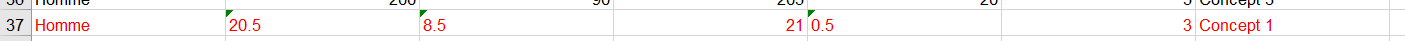
\includegraphics[width=3in]{1.PNG}
   % 	\caption{text}
    \end{figure}          
 \vspace{1.5in}
}



\author{\textbf{\hmwkAuthorName}\\
\textbf{\autre}\\
\textbf{\auttre}\\
}

\date{}

\renewcommand{\part}[1]{\textbf{\large Part \Alph{partCounter}}\stepcounter{partCounter}\\}

%
% Various Helper Commands
%

% Useful for algorithms
\newcommand{\alg}[1]{\textsc{\bfseries \footnotesize #1}}

% For derivatives
\newcommand{\deriv}[1]{\frac{\mathrm{d}}{\mathrm{d}x} (#1)}

% For partial derivatives
\newcommand{\pderiv}[2]{\frac{\partial}{\partial #1} (#2)}

% Integral dx
\newcommand{\dx}{\mathrm{d}x}

% Alias for the Solution section header
\newcommand{\solution}{\textbf{\large Solution}}

% Probability commands: Expectation, Variance, Covariance, Bias
\newcommand{\E}{\mathrm{E}}
\newcommand{\Var}{\mathrm{Var}}
\newcommand{\Cov}{\mathrm{Cov}}
\newcommand{\Bias}{\mathrm{Bias}}

\begin{document}

\maketitle
\pagebreak	
\newpage
\begin{center}
\Huge\textbf{Table des matières}
\end{center}
\tableofcontents
\pagebreak



\section{Introduction}
Le microcontrôleur choisi est-il en accord avec le CDC du ROBI2021 ?\\
Pour repondre cette question, on va travailler sur les 4 exigences qui sont dans la cahier de charge. Afin de realiser les fonctions, on a simule les signals d'entrees et des sorties.\\

\begin{itemize}
\item On remplace les entrees des capteurs par ADCs
\item On remplace les sorties des vitesses par le nombre de Leds qui allument
\end{itemize}
On va étudier, évaluer et mettre en œuvre le microcontrôleur choisi par l’équipe de développement afin d’être intégré au ROBI2021.






\pagebreak
\section{Analyse}
Pour chaque exigence, on doit definir l'entree et la sortie.
\begin{itemize}
	\item \textbf{Exigence 1 Pilotage par l’utilisateur}\\
L’utilisateur pilotera ce chariot à l’aide d’une commande filaire munie de deux boutons : Sens 1 soit de A vers B et Sens 2 soit de B vers A.
\end{itemize}
Pour changer les sens, il faut mettre deux boutons pour ``A gauche" ou ``A droit". En plus, on ajourte un bouton pour arreter la voiture. Pour que la changement de sens soit achronizoique, les entrees doit realise par ``interrupt".
\begin{table}[htbp]
\centering
\begin{tabular}[h]{|c|c|c|c|}
	\hline
	RB4&E&N&Changer le sens comme A droit\\
	\hline
	RB5&E&N&Changer le sens comme A gauche\\
	\hline
	RB3&E&N&Arreter la voiture\\
	\hline
	RA1&S&N&Afficher le sens comme A droit\\
	\hline
	RA2&S&N&Afficher le sens comme A gauche\\
	\hline
\end{tabular}
\end{table}




\begin{itemize}	
	\item \textbf{Exigence 2 Vitesse de déplacement du chariot}\\
La distance di entre le chariot et les butées placées aux points A et B mais aussi avec d’éventuels obstacles sera mesurée. Dans un premier temps, nous validerons le principe de fonctionnement suivant sur un seul sens de déplacement avant de l’implémenter sur les deux sens. 
\end{itemize}
Pour que deux ADCs qui doit etre utilise pour deux capteurs soient independants, on utilise deux entrees.


\begin{table}[htbp]
\centering
\begin{tabular}[h]{|c|c|c|c|}
	\hline
	RA0&E&A&1eme capteur\\
	\hline
	RB0&E&A&1eme capteur\\
	\hline
	RC0-7&S&N&Afficher l'information de la vitesse\\
	\hline
\end{tabular}
\end{table}


\begin{itemize}	
	\item \textbf{Exigence 3 Mesure vitesse de déplacement et régulation}\\
	La vitesse de rotation du moteur sera déduite à l’aide d’un capteur numérique, capteur comptant le nombre de tours du moteur.
\end{itemize}
Pour mesurer la vitesse de la rotation, il faut utiliser un ``interrupt" pour mesurer le nombre de tours et un ``Timer0" pour mesurer le temps passe.
\begin{table}[htbp]
	\centering
\begin{tabular}[h]{|c|c|c|c|}
	\hline
	RB1&E&A&Captueur de rotation\\
	\hline
	RD0-7&S&N&Afficher l'information de la vitesse\\
    \hline
\end{tabular}
\end{table}

\pagebreak
\textbf{\underline{En conclusion:}}
\begin{table}[htbp]
	\centering
	\begin{tabular}[h]{|c|c|c|c|c|c|c|c|c|}
		\hline
	    Nom du registre&b7&b6&b5&b4&b3&b2&b1&b0\\
	    \hline
	    TRISA&x&x&x&x&x&0&0&1\\
	    \hline
	    ANSEL&x&x&x&x&x&0&0&1\\
	    \hline
	    PORTA&0&0&0&0&0&0&0&0\\
	    \hline
	    TRISB&x&x&1&1&1&x&1&1\\
	     \hline
	    ANSELH&x&x&0&1&0&0&0&x\\
	     \hline
	    PORTB&0&0&0&0&0&0&0&0\\
	     \hline
	    TRISC&0&0&0&0&0&0&0&0\\
	     \hline
	    PORTC&0&0&0&0&0&0&0&0\\
	     \hline
	    TRISD&0&0&0&0&0&0&0&0\\
	     \hline
	    PORTD&0&0&0&0&0&0&0&0\\
	     \hline
	\end{tabular}
\end{table}

\text{port:}
\begin{lstlisting}[frame=shadowbox]
PORTA = 0;
PORTB = 0;
PORTC = 0;
PORTD = 0;
\end{lstlisting}
\text{Pour A}
\begin{lstlisting}[frame=shadowbox]
TRISA.TRISA1 = 0;   /***Deux sorties pour afficher l'information de sens ***/
TRISA.TRISA2 = 0;
TRISA.TRISA0 = 1;   /***Entree de ADC  ***/
ANSEL.ANS0 = 1;
ANSEL.ANS1 = 0;
ANSEL.ANS2 = 0;
PORTA.RA1 = 0;    /****** sens initial****/
PORTA.RA2 = 0;
\end{lstlisting}
\text{Pour B}
\begin{lstlisting}[frame=shadowbox]
TRISB.TRISB5 = 1;     /** Deux entree pour changer les sens****/
TRISB.TRISB4 = 1;
ANSELH.ANS11 = 0;    /** Deux entree numeriques***/
ANSELH.ANS13 = 0;
TRISB.TRISB3 = 1;  /*** pour arrete**/
ANSELH.ANS9 = 0;
TRISB.TRISB0 = 1;     /**l'entree de ADC**/
ANSELH.ANS12 = 1;
TRISB.TRISB1 = 1;       // RB1 : entree du interrupt pour calculer le nombre de temps
ANSELH.ANS10 = 0;
\end{lstlisting}
\text{Pour C}
\begin{lstlisting}[frame=shadowbox]
/** 8 sorties pour realiser la vitesse sera proportionnelle a la distance d mesuree**/
TRISC.TRISC0 = 0;
TRISC.TRISC1 = 0;
TRISC.TRISC2 = 0;
TRISC.TRISC3 = 0;
TRISC.TRISC4 = 0;
TRISC.TRISC5 = 0;
TRISC.TRISC6 = 0;
TRISC.TRISC7 = 0;
\end{lstlisting}
\text{Pour D}
\begin{lstlisting}[frame=shadowbox]
/** 8 sorties pour realiser la vitesse sera proportionnelle a la distance d mesuree**/
TRISD.TRISD0 = 0;
TRISD.TRISD1 = 0;
TRISD.TRISD2 = 0;
TRISD.TRISD3 = 0;
TRISD.TRISD4 = 0;
TRISD.TRISD5 = 0;
TRISD.TRISD6 = 0;
TRISD.TRISD7 = 0;
\end{lstlisting}








\pagebreak
\section{Changement du sens}
Afin de changer de sens ouu bien arreter la voiture, on doit configurer sur ``interrupt":
    \begin{figure}[H]
	\centering
	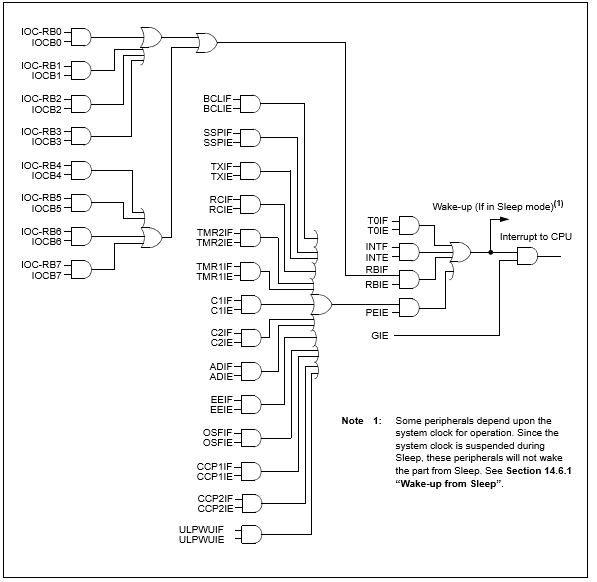
\includegraphics[width=6in]{3.PNG}
	% 	\caption{text}
\end{figure} 
Pour envoyer les infors a CPU, il faut mettre tous les IOCB comme 0 sauf qu'on va utiliser. D'apres la figure au dessus, on configure interrupt:
\begin{lstlisting}[frame=shadowbox]
/**** interrupt configuration ****/
IOCB = 0;            
INTCON.GIE = 1;
INTCON.RBIF = 0;
INTCON.RBIE = 1;
IOCB.IOCB5 = 1;
IOCB.IOCB4 = 1;
IOCB.IOCB3 = 1;
\end{lstlisting}
Apres configurer. On met la fonction suivant pour donner un signal de changer du sens:
\begin{lstlisting}[frame=shadowbox]
bit Change_sens;
void interrupt()       /***interrupt pour changer les sens et counter les tours***/
{
if(INTCON.RBIF == 1)
{
if(PORTB.RB5 == 1|PORTB.RB4 == 1|PORTB.RB3 == 1)
{
Change_sens = 1;
}
INTCON.RBIF = 0;
}
}
\end{lstlisting}
Si on obtient Change\_sens = 1, on va continuer la fonction dans main{}:
\begin{lstlisting}[frame=shadowbox]
void main() {
do
{
 if(Change_sens == 1 && PORTB.RB5 == 1 && PORTB.RB4 == 0)            /**** Changer les sens ***/
{
PORTA.RA2 = 1;
PORTA.RA1 = 0;
Change_sens = 0;
}
if(Change_sens == 1 && PORTB.RB4 == 1 && PORTB.RB5 == 0)
{
PORTA.RA2 = 0;
PORTA.RA1 = 1;
Change_sens = 0;
}
if(Change_sens == 1 && PORTB.RB3 == 1)
{
PORTA.RA2 = 0;
PORTA.RA1 = 0;
Change_sens = 0;
}
}while(1);
}
\end{lstlisting}
\pagebreak
\section{Realisation le contrôle de la vitesse}
Afin d' utiliser ADC, on doit configurer d'abord:
   



\begin{lstlisting}[frame=shadowbox]
/***ADC  ADCON configuration **/
ADCON0.ADCS0 = 0;        /**ADCS1 = 1 ADCS0 = 0  C-a-dire 8HZ 32bits**/
ADCON0.ADCS1 = 1;
ADCON0.CHS0 = 0;      /**entree est A0, du coup 0000*/
ADCON0.CHS1 = 0;
ADCON0.CHS2 = 0;
ADCON0.CHS3 = 0;
ADCON0.GO = 0;     /**GO DONE = 0     **/
ADCON0.ADON = 1;    /**ADON = 1 ADC is enable**/

ADCON1.VCFG0 = 0;           /** l'entree**/
ADCON1.VCFG1 = 0;           /** connecter la masse**/
ADCON1.ADFM = 1;        /**ADFM = 1 **/

/***** Configuration des comparateurs *****/

C1ON_bit = 0;                    // Disable all comparators
C2ON_bit = 0;                    //PWM
\end{lstlisting}
En suite, il faut creer une fonciton de ADC:
\begin{lstlisting}[frame=shadowbox]
unsigned ReadADC1 (void);       /**** Commencer ADC pour les capteurs distances **/
unsigned ReadADC2 (void);
void main() {          
unsigned res1 = 0;                // result of analog to digital conversion
unsigned res2 = 0;
do
{
res1 = ReadADC1();
res2 = ReadADC2();
/***On choisi dmin est 20% de distance total, et c'est presque 200/1023**/
if(res1 < 50)
{
PORTC.RC0 = 0;
PORTC.RC1 = 0;
PORTC.RC2 = 0;
PORTC.RC3 = 0;
}
if(51 <= res1 && res1 < 100)
{
PORTC.RC0 = 1;
PORTC.RC1 = 0;
PORTC.RC2 = 0;
PORTC.RC3 = 0;
}
if(101 <= res1 && res1 < 150)
{
PORTC.RC0 = 1;
PORTC.RC1 = 1;
PORTC.RC2 = 0;
PORTC.RC3 = 0;
}
if(151 <= res1 && res1 < 200)
{
PORTC.RC0 = 1;
PORTC.RC1 = 1;
PORTC.RC2 = 1;
PORTC.RC3 = 0;
}
if(res1 >= 200)
{
PORTC.RC0 = 1;
PORTC.RC1 = 1;
PORTC.RC2 = 1;
PORTC.RC3 = 1;
}
if(res2 < 50)
{
PORTC.RC4 = 0;
PORTC.RC5 = 0;
PORTC.RC6 = 0;
PORTC.RC7 = 0;
}
if(51 <= res2 && res2 < 100)
{
PORTC.RC4 = 1;
PORTC.RC5 = 0;
PORTC.RC6 = 0;
PORTC.RC7 = 0;
}
if(101 <= res2 && res2 < 150)
{
PORTC.RC4 = 1;
PORTC.RC5 = 1;
PORTC.RC6 = 0;
PORTC.RC7 = 0;
}
if(151 <= res2 && res2 < 200)
{
PORTC.RC4 = 1;
PORTC.RC5 = 1;
PORTC.RC6 = 1;
PORTC.RC7 = 0;
}
if(res2 >= 200)
{
PORTC.RC4 = 1;
PORTC.RC5 = 1;
PORTC.RC6 = 1;
PORTC.RC7 = 1;
}
}while(1);
}
unsigned ReadADC1(){
unsigned res1;

ADCON0.CHS0 = 0;      /**entree est A0, du coup 0000*/
ADCON0.CHS1 = 0;
ADCON0.CHS2 = 0;
ADCON0.CHS3 = 0;

Delay_us(4);

ADCON0.GO = 1;      // start conversion comme go
while(ADCON0.GO == 1){};
res1 = ADRESH * 256 + ADRESL;
return res1;
}


unsigned ReadADC2() {
unsigned res2;
ADCON0.CHS0 = 0;      //entree est B0, du coup 1100
ADCON0.CHS1 = 0;
ADCON0.CHS2 = 1;
ADCON0.CHS3 = 1;

Delay_us(4);


ADCON0.GO = 1;      // start conversion comme go
while(ADCON0.GO == 1){};

res2 = ADRESH * 256 + ADRESL;
return res2;
}
\end{lstlisting}
















\pagebreak
\section{Mesure de vitesse de la rotation}
\textbf{La vitesse de rotation du moteur sera déduite à l’aide d’un capteur numérique, capteur comptant le nombre de tours du moteur.}\\

Afin de réaliser cette fonction, on utilise méthode de ``interrupt" pour la mesure du nombre de rotations et méthode de ``Timer0" pour la mesure du temps passés.

\begin{figure}[H]
	\centering
	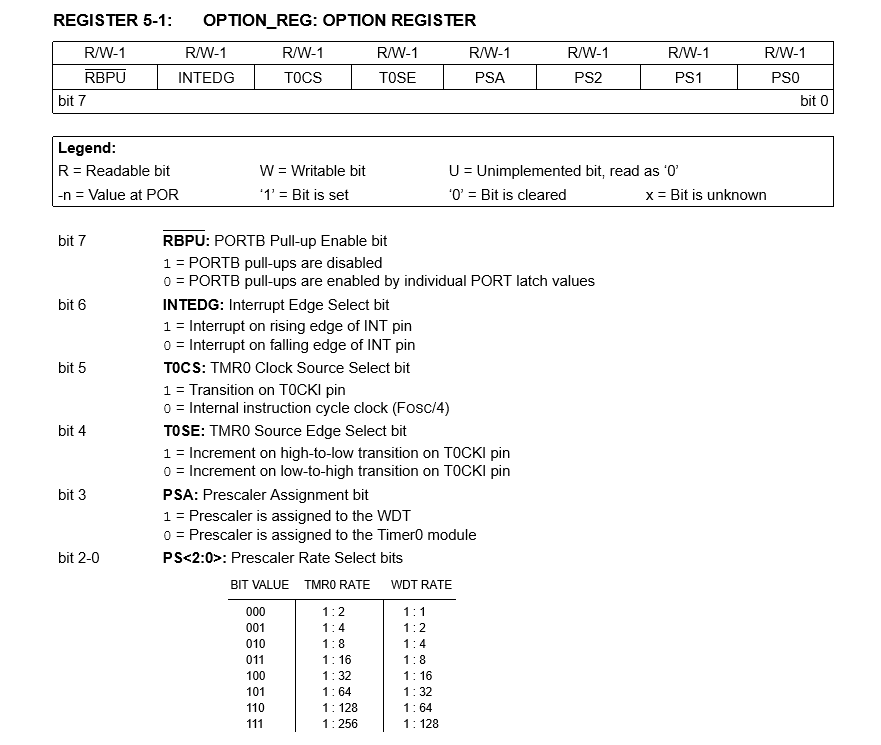
\includegraphics[width=6in]{2.PNG}
	% 	\caption{text}
\end{figure} 
Pour la configuration de Timer0, comme la figure ci-dessus. On doit prendre ``Internal instruction cycle clock (Fosc/4)" et ``Prescaler is assigned to the Timer0 module". C'est à dire, on met OPTION\_REG.T0CS = 0 et OPTION\_REG.PSA = 0; Pour $PS<2:0>$, on choisi 1:64. Comme le code suivant:
\begin{lstlisting}[frame=shadowbox]
OPTION_REG.PS0 = 1;   
OPTION_REG.PS1 = 0;
OPTION_REG.PS2 = 1;
OPTION_REG.PSA = 0;  // Prescaler is assigned to the Timer0 module
OPTION_REG.T0CS = 0;   //Internal instruction cycle clock (Fosc/4)
\end{lstlisting}
\pagebreak
Pour la configuration de ``interrupt". On prend un input \textbf{RB1} comme la capteur de la rotation. Donc comme la 2eme exigence, on complete la code de la configuration de ``interrupt".
\begin{lstlisting}[frame=shadowbox]
IOCB = 0;          
IOCB.IOCB1 = 1;   
INTCON.GIE = 1;
INTCON.RBIF = 0;
INTCON.RBIE = 1;
INTCON.T0IE = 1;   //Repondre au besoin de Timer0
INTCON.T0IF = 1;
\end{lstlisting}
On a choisi 1:64 comme Prescaler Rate Select bits.
\begin{align*}
T_{inc} &= T_{osc}*4*64 \\
T_{deb} &= T_{inc}*256 \\
N_{deb} &= \frac{1}{T_{deb}} = 123
\end{align*}
On a 123 fois de debordements chaque second.
\begin{lstlisting}[frame=shadowbox]
int count_tours;
int cot;
int time;
void interrupt()                           
{
	if(INTCON.RBIF == 1)
	{
		if(PORTB.RB1 == 1)     //le capteur
		{
			count_tours ++ ;
		}
		INTCON.RBIF = 0;
	}
	if(INTCON.T0IF == 1)      // debortement
	{
		time ++;
		if(time > 123)    //une seconde
		{
		cot = count_tours;       // cot: vitesse de la rotation par seconde
		count_tours = 0;
		time = 0;
		} 
		INT0IF_bit = 0;
	}
}
\end{lstlisting}
Pour valider cette fonction, on met le code suivant dans do\{\}while\{1\}; Comme ca, on peut tester la fonction.
\begin{lstlisting}[frame=shadowbox]
PORTD = cot;
\end{lstlisting}
\pagebreak

\section{Conclusion}
Comme le travail avant, on a reussi de realiser les fonctions. On touve des problems comme:
\begin{itemize}
 \item Les leds qui sont utilises pour afficher les informations sont insuffisants.
 \item Pour que les entrees soient automatiques, par exemple le capteur de rotation, il faut trouver comment passer le signal a la carte (pour remplacer appuyer sur les buttons tout le temps).
 \item On doit brancher l'ecran sur le portC et le portD donc on peut savoir la vitesse.
 \item Dans 2eme exigencce, on doit configurer sur PWM pour commander le moteur.
\end{itemize}

En conclusion, la carte qu'on a choisi est suffisant pour les 4 exigences pour l'instant mais il faut travailler plus pour completer les fonctions.



\end{document}
